\vspace{2mm}




\tikzset{every picture/.style={line width=0.75pt}} %set default line width to 0.75pt        

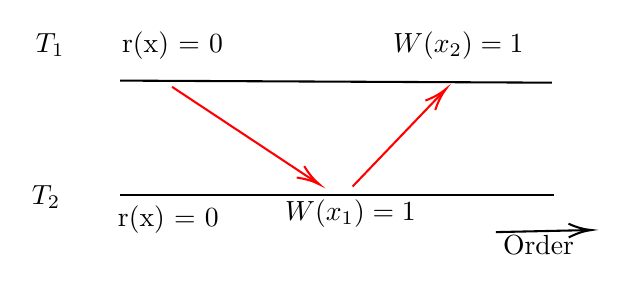
\begin{tikzpicture}[x=0.75pt,y=0.75pt,yscale=-1,xscale=1]
%uncomment if require: \path (0,300); %set diagram left start at 0, and has height of 300

%Straight Lines [id:da9500410641573396] 
\draw    (63.56,64) -- (271.56,65) ;
%Straight Lines [id:da7796185686481738] 
\draw    (63.56,119) -- (272.56,119) ;
%Straight Lines [id:da7329480179958066] 
\draw    (244.56,137) -- (288.56,136.04) ;
\draw [shift={(290.56,136)}, rotate = 178.75] [color={rgb, 255:red, 0; green, 0; blue, 0 }  ][line width=0.75]    (10.93,-3.29) .. controls (6.95,-1.4) and (3.31,-0.3) .. (0,0) .. controls (3.31,0.3) and (6.95,1.4) .. (10.93,3.29)   ;
%Straight Lines [id:da06917928011783969] 
\draw [color={rgb, 255:red, 255; green, 0; blue, 0 }  ,draw opacity=1 ]   (88.56,67) -- (157.89,112.9) ;
\draw [shift={(159.56,114)}, rotate = 213.5] [color={rgb, 255:red, 255; green, 0; blue, 0 }  ,draw opacity=1 ][line width=0.75]    (10.93,-3.29) .. controls (6.95,-1.4) and (3.31,-0.3) .. (0,0) .. controls (3.31,0.3) and (6.95,1.4) .. (10.93,3.29)   ;
%Straight Lines [id:da061796007668484476] 
\draw [color={rgb, 255:red, 255; green, 0; blue, 0 }  ,draw opacity=1 ]   (175.56,115) -- (219.18,69.44) ;
\draw [shift={(220.56,68)}, rotate = 133.75] [color={rgb, 255:red, 255; green, 0; blue, 0 }  ,draw opacity=1 ][line width=0.75]    (10.93,-3.29) .. controls (6.95,-1.4) and (3.31,-0.3) .. (0,0) .. controls (3.31,0.3) and (6.95,1.4) .. (10.93,3.29)   ;

% Text Node
\draw (21.5,40) node [anchor=north west][inner sep=0.75pt]   [align=left] {$T_1$};
% Text Node
\draw (19.5,113) node [anchor=north west][inner sep=0.75pt]   [align=left] {$T_2$};
% Text Node
\draw (141.56,120) node [anchor=north west][inner sep=0.75pt]   [align=left] {$W(x_1) = 1$};
% Text Node
\draw (63,39) node [anchor=north west][inner sep=0.75pt]   [align=left] {r(x) = 0};
% Text Node
\draw (246.56,137) node [anchor=north west][inner sep=0.75pt]   [align=left] {Order};
% Text Node
\draw (193.56,39) node [anchor=north west][inner sep=0.75pt]   [align=left] {$W(x_2)=1$};
% Text Node
\draw (61,123) node [anchor=north west][inner sep=0.75pt]   [align=left] {r(x) = 0};


\end{tikzpicture}

\vspace{2mm}

\begin{equation}
History\ H: [R_1(x_0),R_2(x_0),W_2(x=1),W_1(x=1)]
\end{equation}
\vspace{2mm}